\section{Transistor-Transistor-Logik}

\begin{itemize}
    \item Meist statischer Stromverbrauch
    \item Asymmetrische Schaltschwellen (weniger Marge als CMOS-Logik)
\end{itemize}


\subsection{Resistor Transistor Logik (RTL)}

\begin{minipage}[c]{0.27\columnwidth}
    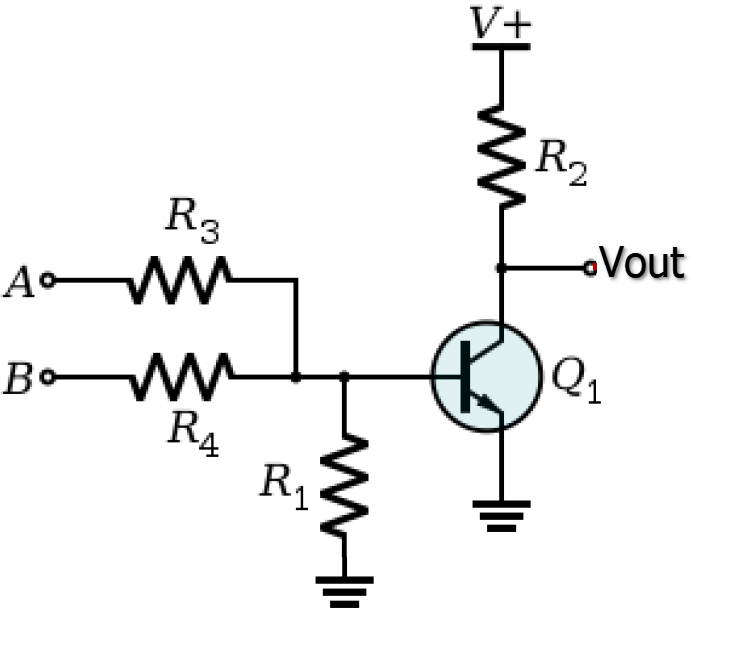
\includegraphics[width=\columnwidth]{images/rtl_nor.png}
\end{minipage}
\hfill
\begin{minipage}[c]{0.68\columnwidth}
    Bild: NOR-Gate

    \begin{itemize}
        \item Ausgangsspannung $V_{\rm out} = V_+$ oder $V_{\rm out} = V_{\rm CE,sat}$
        \item \textbf{Fan-Out ist begrenzt} (Werden zu viele weitere Gatter an den Ausgang gehängt, so reicht der Strom nicht mehr,
             um diese zu treiben \textrightarrow\ Spannungslevel stimmen nicht mehr, um Transisoren durchzusteuern)
    \end{itemize}
\end{minipage}


\subsection{Dioden-Transistor-Logik (DTL)}

\begin{minipage}[c]{0.3\columnwidth}
    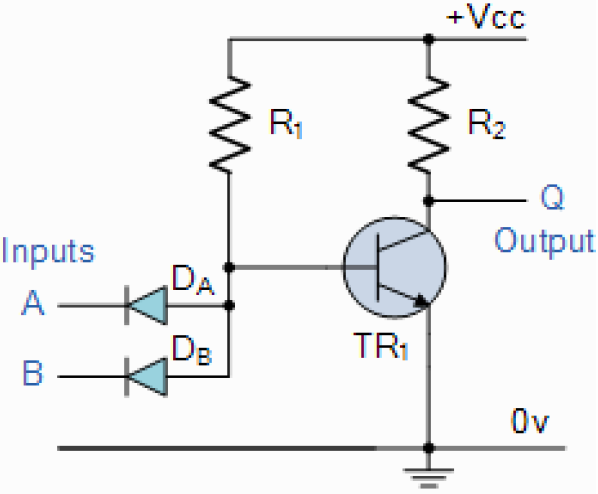
\includegraphics[width=\columnwidth]{images/dtl_nand_gate.png}
\end{minipage}
\hfill
\begin{minipage}[c]{0.68\columnwidth}
    Bild: NAND-Gate

    \begin{itemize}
        \item \textbf{Fan-Out grösser}, da Transistor aktiv nach '0' zieht
        \item $R_2$ muss keine Gatter treiben (kein grosser Stromfluss)
        \item Nachteile: Sehr tiefer Störabstand; Transistor leitet schon bei Spannungen, welche kaum $> 0 \, \volt$ sind 
    \end{itemize}
\end{minipage}


\subsection{Transistor-Transistor-Logik (TTL)}

\begin{minipage}[c]{0.3\columnwidth}
    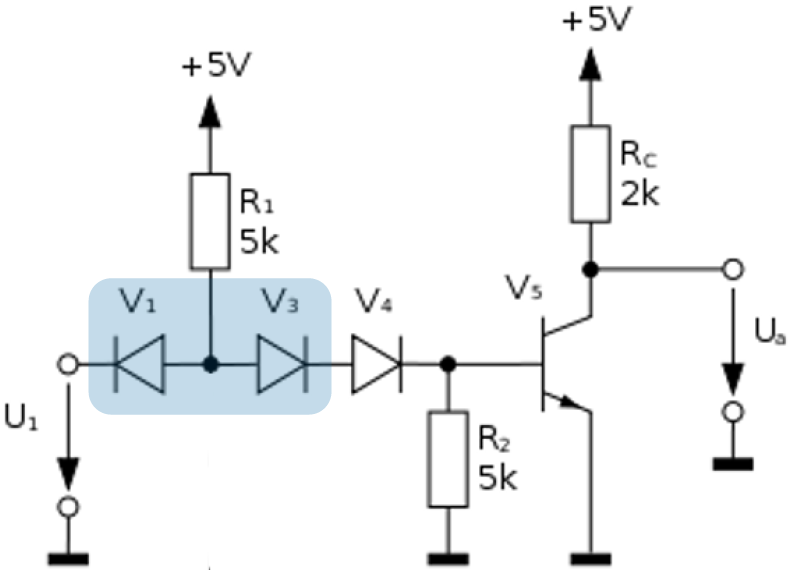
\includegraphics[width=\columnwidth]{images/dtl_zu_ttl.png}
\end{minipage}
\hfill
\begin{minipage}[c]{0.11\columnwidth}
    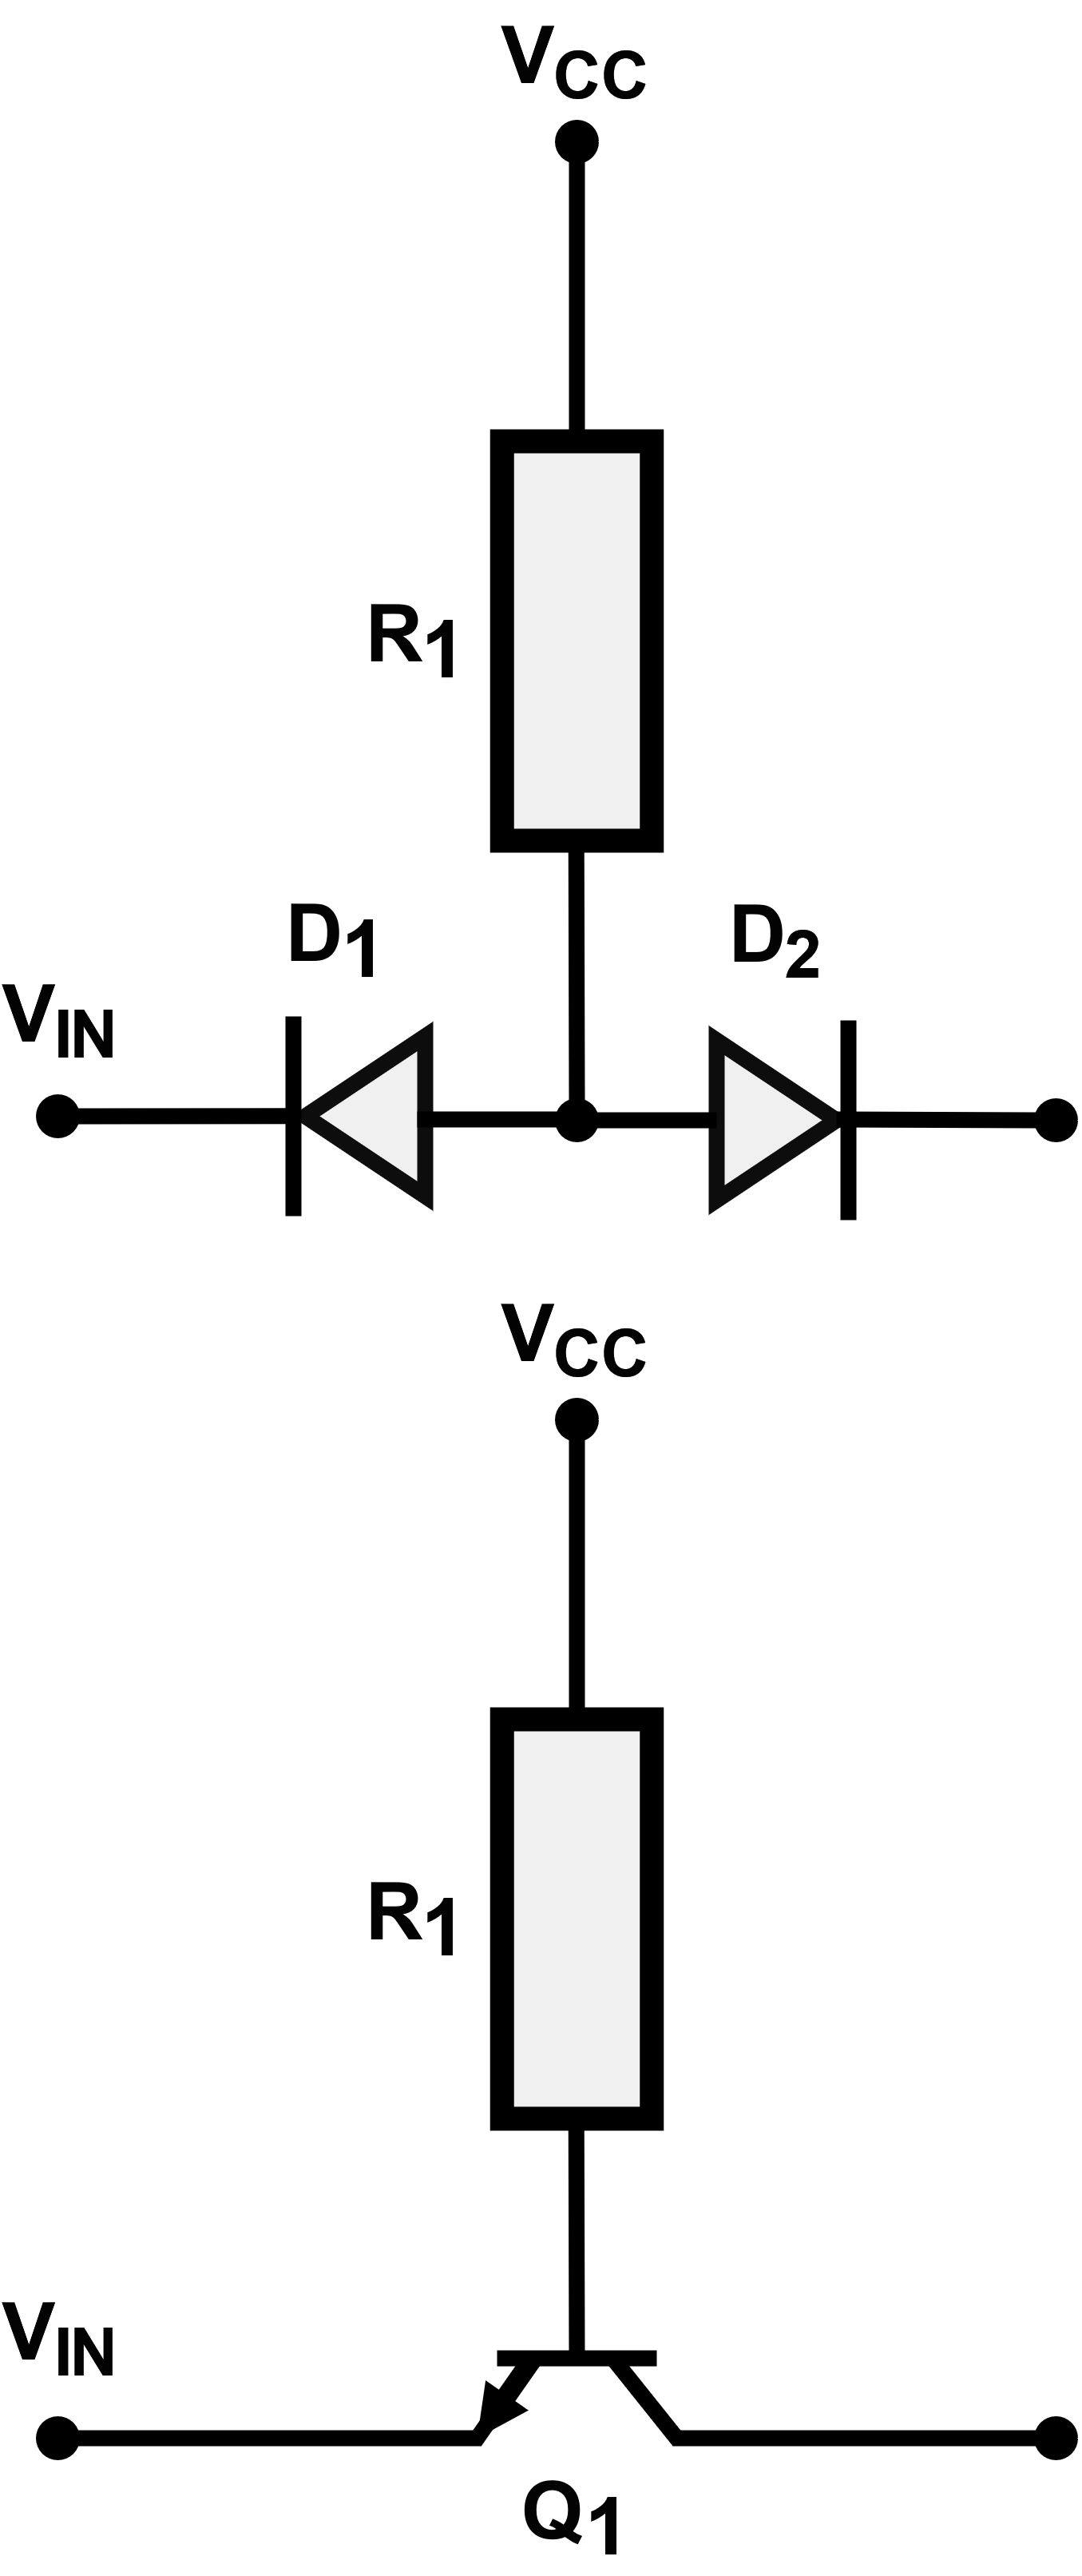
\includegraphics[width=\columnwidth]{images/dtl_diodes_transistor.png}
\end{minipage}
\hfill
\begin{minipage}[c]{0.48\columnwidth}
    \begin{itemize}
        \item  Schaltschwelle am Eingang wird durch Dioden $V_3$ und $V_4$ um $1.4 \, \volt$ erhöht
        \item Dioden $V_1$ und $V_3$ bilden npn-Struktur \textrightarrow\ npn-Transistor
    \end{itemize}
\end{minipage}

